%This is my super simple Real Analysis Homework template
\documentclass[a4paper]{book}

%% Language and font encodings
\usepackage[T1,T8K,T8M]{fontenc}
\usepackage[utf8]{inputenc}
\usepackage[english,georgian]{babel}

%% Sets page size and margins
\usepackage[a4paper,top=3cm,bottom=2cm,left=3cm,right=3cm,marginparwidth=1.75cm]{geometry}

\usepackage[plainpages=false,bookmarksopen,pdfpagelabels, %
pdftex,
pdfproducer={Latex with hyperref},
pdfcreator={pdflatex},
bookmarksnumbered,unicode]{hyperref} 



%% Useful packages
\usepackage{amsmath}
\usepackage{graphicx}
\usepackage[colorinlistoftodos]{todonotes}
%\usepackage[colorlinks = true, allcolors = blue]{hyperref}
\usepackage{float}
\usepackage{enumerate}
\usepackage{subfig}
\usepackage{gensymb}
\usepackage{rotating}
\usepackage[version=4]{mhchem}


\title{ფიზიკა}
\author{ლევან კანკაძე}

\begin{document}
\maketitle

\tableofcontents

\chapter{წინასიტყვაობა.}
\chapter{ელექტრობა და მაგნეტიზმი}
\textbf{3.57} სურათზე \ref{fig:3_57} გამოსახული უსასრულო წრედი შედგება ერთნაირი ელემენტებისა და ვოლტმეტრებისაგან. ყველაზე მარცხენა ვოლტმეტრის ჩვენებეაა $U$, ხოლო ყოველი შემდეგის ჩვენება $n$ჯერ ნაკლებია, ვიდრე მის მარცხენა მეზობელზე ($n>1$). იპოვეთ ელემენტის ემძ.


	\begin{figure}[H]
		\centering
		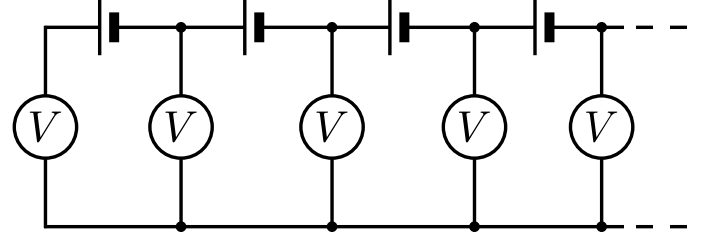
\includegraphics[width=0.2\columnwidth]{images/3_57}
		\caption{ამოცანა 3.57.}
		\label{fig:3_57}
	\end{figure}

\end{document}